\documentclass[12pt]{article}
\usepackage{geometry}
\geometry{letterpaper}

\newcommand{\hide}[1]{}
\newcommand{\exercisea}{\texttt{exercisea.py}\;}
\newcommand{\exercisec}{\texttt{exercisec.py}\;}
\newcommand{\exercised}{\texttt{exercised.py}\;}
\newcommand{\exercisee}{\texttt{exercisee.py}\;}


\renewcommand\thesubsection{\thesection.\alph{subsection}}

\usepackage{xcolor}
\usepackage{url}
\usepackage{hyperref}
\usepackage{mathtools}
\usepackage{graphicx}
\usepackage[labelfont=bf]{caption}
\usepackage{subcaption}

\hide{
\usepackage{amscd}
\usepackage{amsfonts}
\usepackage{amsmath}
\usepackage{amssymb}
\usepackage{amsthm}
\usepackage{cases}		 
\usepackage{cutwin}
\usepackage{enumerate}
\usepackage{epstopdf}
\usepackage{graphicx}
\usepackage{ifthen}
\usepackage{lipsum}
\usepackage{mathrsfs}	
\usepackage{multimedia}
\usepackage{wrapfig}
}

	 
%\input{/usr/local/LATEX/Lee_newcommands.tex}
\newcommand{\itemlist}[1]{\begin{itemize}#1\end{itemize}}
\newcommand{\enumlist}[1]{\begin{enumerate}#1\end{enumerate}}
\newcommand{\desclist}[1]{\begin{description}#1\end{description}}

\newcommand{\Answer}[1]{\begin{quote}{\color{blue}#1}\end{quote}}
\newcommand{\AND}{\wedge}
\newcommand{\OR}{\vee}
\newcommand{\ra}{\rightarrow}
\newcommand{\lra}{\leftrightarrow}

\title {Crash Course Deep Learning - Assignment 1}
\author{Instructor:  Prof. Alexander Sch\"onhuth \\ Submitted by: Jan Gerrit H\"olting \\ Student ID: 6570518 \\ Universiteit Utrecht}
\date{}

\begin{document}
\maketitle

In this assignment, we will perform an experimental analysis of basic neural networks and the effect of different choices of hyperparameters on their performance. The test data set for the neural network will in each case be the MNIST database of handwritten digits (see \cite{MNIST}) containing 60,000 training examples as well as 10,000 test examples. The experimental results have been obtained using the accompanying Python implementation which in turn uses Google's open-source machine learning platform TensorFlow 2 (see \cite{TensorFlow}).\\

\noindent \textbf{General setup:} \\
Some parameters of the neural network will remain constant throughout the following experiments. For more information on the interpretation of the parameters as well as the methods used, the reader is asked to consult Nielsen's \textit{Neural Networks and Deep Learning} \cite{Nielsen} for an informal or Goodfellow et al.s' \textit{Deep Learning} \cite{Goodfellow} for a more formal introduction. We will use 50 epochs, a batch size of 100 while iterating through the example data, 5-fold cross validation as well as a standard gradient descent optimzer with a learning rate of 0.5. In the output layer we will use cross entropy as the loss function with softmax activation while all hidden layers will use the sigmoid function as the activation function. Furthermore, the number 6570518 is used as a seed for both the cross-validation as well as the for the random initialisation of the weights and biases.

Clearly, all of the above choices can independently be subjected to hyperparameter tuning. For this report, however, we will restrict ourselves to observing some first experimental results and the differences in performances for different choices of number of layers, number of nodes and additional layer options such as performing a probabilistic drop-out, etc. We will discuss the different choices in each part of the assignment individually. 

\section{Exercises}
\subsection{Creating a basic neural network}
In this part we will outline the structure of a basic neural network (henceforth denoted NN) implemented in Python using TensorFlow. The NN will consists of 3 hidden layers, the first one having 512, the second one 256 and the third one 128 nodes. As stated before, all three layers will use the sigmoid function as the activation function.

The Python implementation is based on TensorFlow 2, using the Keras API. For more information on how to install and import TensorFlow and Keras, the reader is asked to consult \cite{Keras}. The implementation of this first NN can be found in \exercisea and is as structured (on a high level) as follows: we first load the MNIST database and split it in training and test data, the former containing 60,000 data points, the latter 10,000. We then loop through the (random but evenly distributed) splits of the 5-fold cross-validation and in each iteration build and compile the NN and then train it on the training data that is defined by the cross-validation procedure. We then validate the data on a separate set of validation data. Finally, we compute the average performance (test loss and accuracy) of the model on the validation data as well as the performance on the test data.  

\subsection{Evaluating the performance of a basic neural network}\label{sec:b}
The performance of this first NN can be seen in Figure \ref{fig:exercisea}, where the evolution of loss is plotted over the course of the (50) epochs for all 5 splits of training data of the cross-validation. As we can see, the NN performs almost identical on all 5 splits of the training data. A steep decline of loss in the first 10-15 epochs is visible, followed by very little change for the remaining epochs. This suggests that an early abort of the training might be advantageous in order to avoid overfitting and to improve efficiency. The NN has furthermore achieved the following final performance results: on average, the validation loss was 0.096 while the final accuracy on the test data was at 0.98, meaning that 98\% of handwritten digits have been categorised correctly by the NN after 50 epochs of training. We can thus see that this basic neural networks with a large amount of nodes and few layers already achieves a fairly high accuracy after a training period of approximately 20 minutes. 

\begin{figure}[ht]
    \centering
   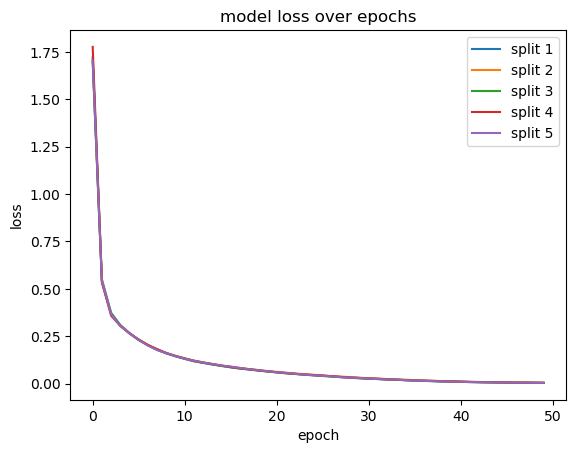
\includegraphics[scale=0.6]{graphics/loss_over_epochs_exercise_a.png}
    \caption{Performance of a NN with three hidden layers of 512, 256 and 128 nodes, respectively: evolution of loss for the different splits of training data over the course of 50 epochs using 5-fold cross-validation.}
    \label{fig:exercisea}
\end{figure}



\subsection{Comparing different NN architectures}\label{sec:comparison}
In this section we will compare different architectures for neural networks in order to determine which model to use for further experimentation. We will compare the following five architectures, all other parameters and functions used will remain the same as explained in the introduction. In particular, all layers will use the sigmoid function as the activation function. 

\begin{enumerate}
    \item one layer with 128 nodes
    \item one layer with 256 nodes
    \item one layer with 512 nodes
    \item two layers with 64 and 32 nodes 
    \item two layers with 256 and 128 nodes
\end{enumerate}

In order to determine which architecture is superior, we will consult the average validation loss, the final accuracy on the test data as well as the time taken for training. We will therefore for each of the five above architectures perform the 5-split cross-validation, collect the loss on each of the five validation data sets and finally average these and analyse the accuracy on the test data set in order to determine the best model. The Python code for this procedure can be found in \exercisec. The results of these experiments can be found in Table \ref{tab:exercisec}. 

\begin{table}[ht]
    \centering
    \begin{tabular}{c|c|c|c}
        \textbf{Model}              & \textbf{Avg. validation loss} & \textbf{Test accuracy} & \textbf{Time (min)} \\ \hline
        1 layer, 128 nodes  &   0.0778 &    0.9786 & 8 \\
        1 layer, 256 nodes  & 0.0746 & 0.9784  & 10   \\
        1 layer, 512 nodes  & 0.0741 & 0.9783 & 12 \\
        2 layers, 64 and 32 nodes   & 0.105 &    0.9738 & 8\\
        2 layers, 256 and 128 nodes & 0.08336 &   0.9787 & 12 
    \end{tabular}
     \caption{Comparing different NN architectures with regard to average validation loss, accuracy on the test data and time taken for training (in minutes).}
        \label{tab:exercisec}
\end{table}

As we can see from the experimental values, all five architectures achieve very similar results for the test accuracy. The do, however, differ greatly in their average validation loss as well as the time taken for training (including all of the cross-validation). Architectures 1, 2 and 3 all seem to perform almost identical with respect to average validation loss and test accuracy, while the avg. validation loss of 4 and 5 are fairly high. It therefore seems reasonable to choose model 2 as the best performing, as it achieves good results on both the avg. validation loss and test accuracy and takes reasonably little time for training. 


\subsection{Applying a probabilistic dropout to the hidden layer}

In this section we will investigate the effect of performing a probabilistic dropout on the nodes of the hidden layer. A dropout operation ignores a node from a hidden layer temporarily and purely by chance according to a given probability, independent of weights or biases associated to that node, so that other nodes will essentially have to step in to account for the representation of that node. In this section, a dropout with probability 0.5 is performed on each node in the hidden layer during each weight updating cycle. For these tests we will use the architecture with one hidden layer containing 256 nodes that we determined in \ref{sec:comparison}. The code for these experiments can be found in \exercised. The plot showing the evolution of loss over the course of the 50 epochs for each of the five splits of the cross-validation can be seen in Figure \ref{fig:exercised}. 

\begin{figure}[ht]
    \centering
   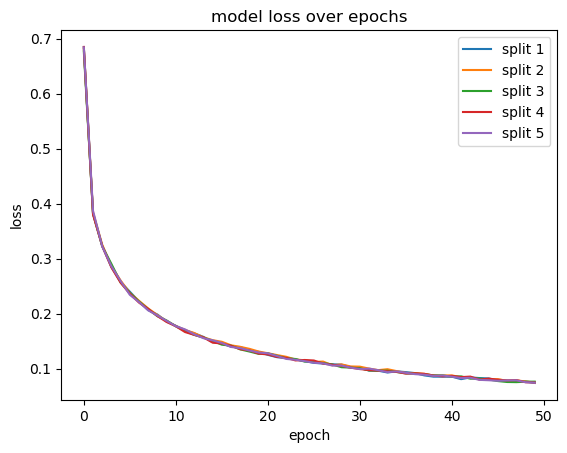
\includegraphics[scale=0.6]{graphics/loss_over_epochs_exercise_d.png}
    \caption{Performance of a NN with one hidden layer of 256 nodes: evolution of loss for the different splits of training data over the course of 50 epochs using 5-fold cross-validation and a dropout of 0.5 for the hidden layer.}
    \label{fig:exercised}
\end{figure}

From the plot we can see that the training loss evolves a little different to that in \ref{sec:b}: it decreases less quickly in the first 20 epochs and overall shows a higher loss compared to \ref{sec:b}. The average validation loss is at 0.08137 while the final test accuracy is 0.9769. We can therefore conclude that applying a dropout with probability 0.5 in this case does not improve the performance of the NN, as both the test accuracy and average validation loss perform worse compared to Section \ref{sec:comparison}.  


\subsection{Adding regularisation to the NN}

For the final section, we will analyse the effect of adding regularisation to the model. In particular, we will investigate the effect of adding l2 regularisation so as to keep the overall weight values small. Note that we will apply the regularisation solely to the weights, not to the biases in each layer. Again, we will perform our analysis on the best model from Section \ref{sec:comparison} containing one layer with 256 nodes. We will not perform any dropout in these experiments. These experiments are implemented in \exercisee. The plot showing the evolution and overall level of training loss over the epochs can be seen in Figure \ref{fig:regularisation}. 

\begin{figure}[ht]
    \centering
   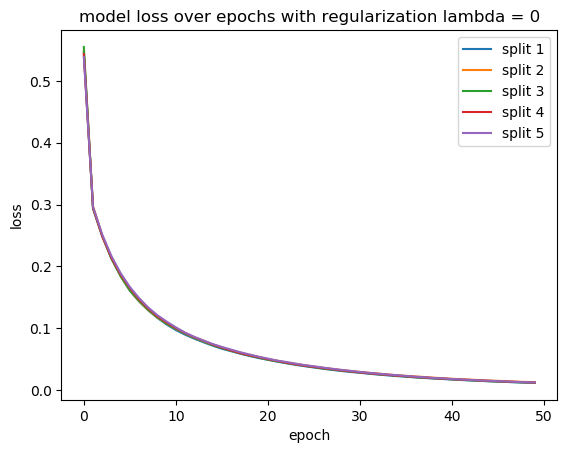
\includegraphics[scale=0.5]{graphics/loss_over_epochs_exercise_e_0.png}
  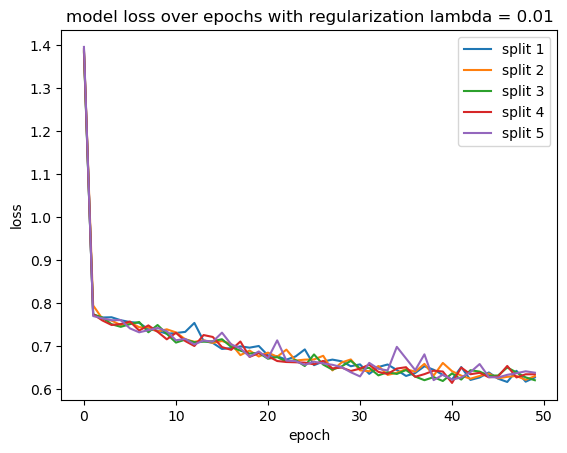
\includegraphics[scale=0.5]{graphics/loss_over_epochs_exercise_e_01.png}
    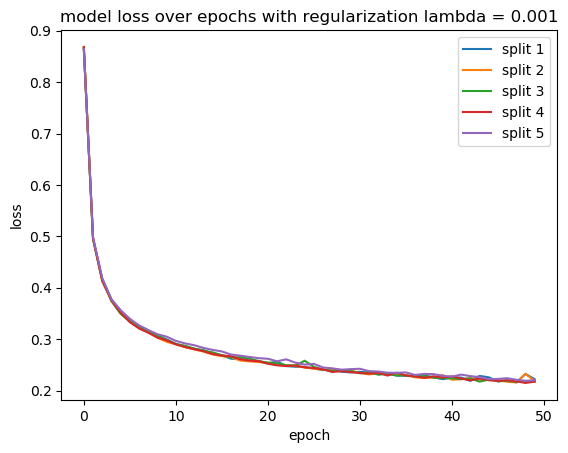
\includegraphics[scale=0.5]{graphics/loss_over_epochs_exercise_e_001.png}
    \caption{Performance of a NN with one hidden layer of 256 nodes: evolution of loss for the different splits of training data over the course of 50 epochs using 5-fold cross-validation and l2 regularisation for different parameters $\lambda$.}
    \label{fig:regularisation}
\end{figure}

As we can see, the overall evolution of loss over the epochs is quite different. While no regularisation and regularisation with $\lambda = 0.001$ have a smooth loss curve and decrease a lot during the first 20 epochs, regularisation with $\lambda = 0.01$ has a very steep loss curve in the first epochs. Moreover, both $\lambda = 0.01$ and $\lambda = 0.001$ have a significantly worse performance with regard to loss compared to no regularisation at all. Overall, applying no regularisation at all seems to significantly outperform applying regularisation for this architecture. This also becomes evident when considering the average validation loss and final test accuracy that can be seen in Figure \ref{fig:regularisation}: overall, the avg. validation is an order of magnitude worse for applying regularisation as compared to $\lambda = 0$. This can also be seen in the test accuracy, that is overall lower than for no regularisation at all. Altogether, we can therefore conclude that applying regularisation for these choices of $\lambda$ does not increase performance of the NN. 

\begin{table}[ht]
    \centering
    \begin{tabular}{c|c|c}
        \textbf{$\lambda$}  & \textbf{Avg. validation loss} & \textbf{Test accuracy} \\ \hline
        0 &   0.07369 & 0.9781  \\
        0.01 & 0.6338 & 0.8961   \\
        0.001 & 0.85544 & 0.9636
    \end{tabular}
     \caption{Average validation loss and test accuracy of a NN with one hidden layer of 256 nodes over the course of 50 epochs using 5-fold cross-validation and l2 regularisation for different parameters $\lambda$.}
        \label{tab:exercisee}
\end{table}




\section{Conclusion}
In the above report we have analysed the performance of several NN architectures for the problem of classifying handwritten digits taken from the MNIST database. We have seen that for this particular problem, a neural network with one hidden layer of 256 nodes might be sufficient and delivers a test accuracy of about 97\% after 50 epochs of training. We have furthermore seen that neither applying a probabilistic dropout nor applying l2 regularisation improves performance of the NN. As hinted in the introduction, there are still a lot of hyperparameters that can be tuned. This, however, would exceed the scope of this first analysis.

\bibliographystyle{alphadin}
\bibliography{DL_1}
\end{document}  